% vim: set filetype=tex spell :

\chapter{Verification}

\label{ch:Verification}

The \ac{ACDS} consists of experimental hardware controlled by experimental software and as such requires a significant amount of verification to make sure everything functions on orbit.

\section{Sensor Verification}

\subsection{Magnetomitor Verification}

The magnetomitor verification is done using the Hemholtz cage 
jj
\subsection{Compensation Testing}

The torquer compensation is tested by running the Helmholtz Cage through a field sequence and taking measurements at each point. During the process a random torquer flip is executed every 10 data points. The measurements are corrected using the compensation data set and compared to the expected field. A typical plot of the data is shown in \cref{fig:tqtst}. The RMS error is also calculated for the data set so the effectiveness of the torquer compensation can be compared to the calibration without torquers.

\begin{figure}[!ht]
    \centering
    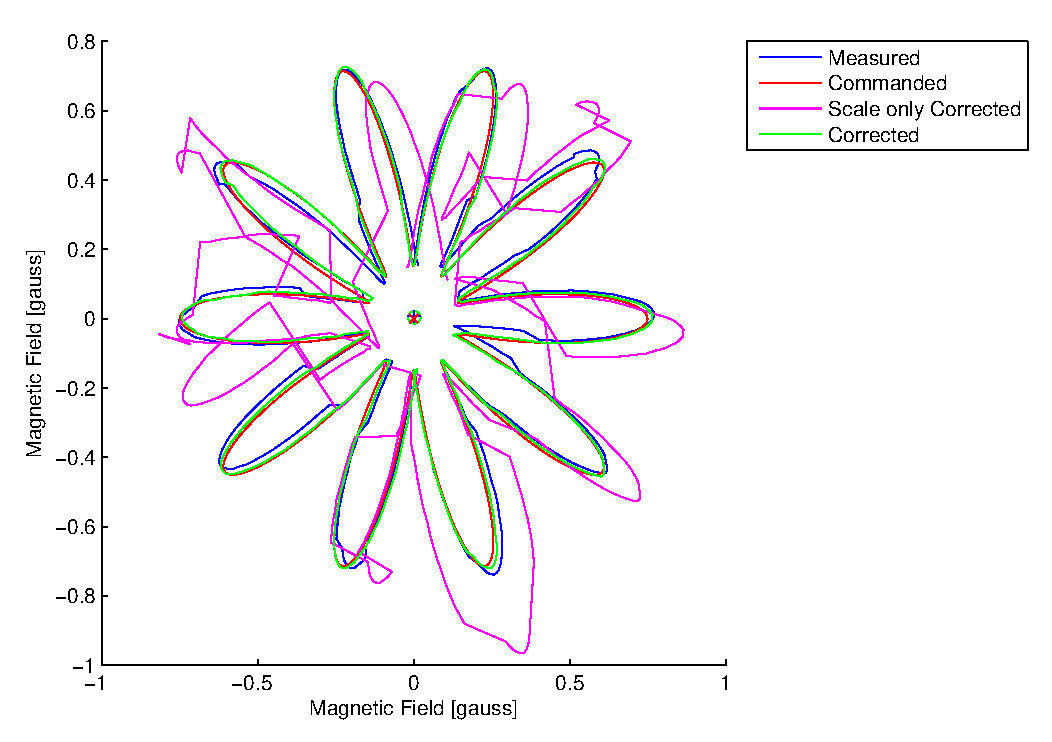
\includegraphics[width=0.8\linewidth]{torqueCalTst}
  \caption{A torquer compensation test showing that the correction provides a large amount of improvement over the uncorrected values}
    \label{fig:tqtst}
\end{figure}

\Cref{fig:tqerr} shows the error for the torquer compensation test. The RMS error for the compensated data is 9 mGauss. The maximum error is 24 mGauss. On a 300 mGauss field a 24 mGauss error will cause an angular error of \textpm5\textdegree. The addition of the torquers causes an increase in the RMS and maximum error.
%This can be seen by comparing \cref{fig:tqerr} with \cref{fig:magerr}. In \cref{fig:tqerr} steps in the error are seen as torquers are flipped whereas in \cref{fig:magerr} the error is more consistent across the entire run.

\begin{figure}[!ht]
    \centering
    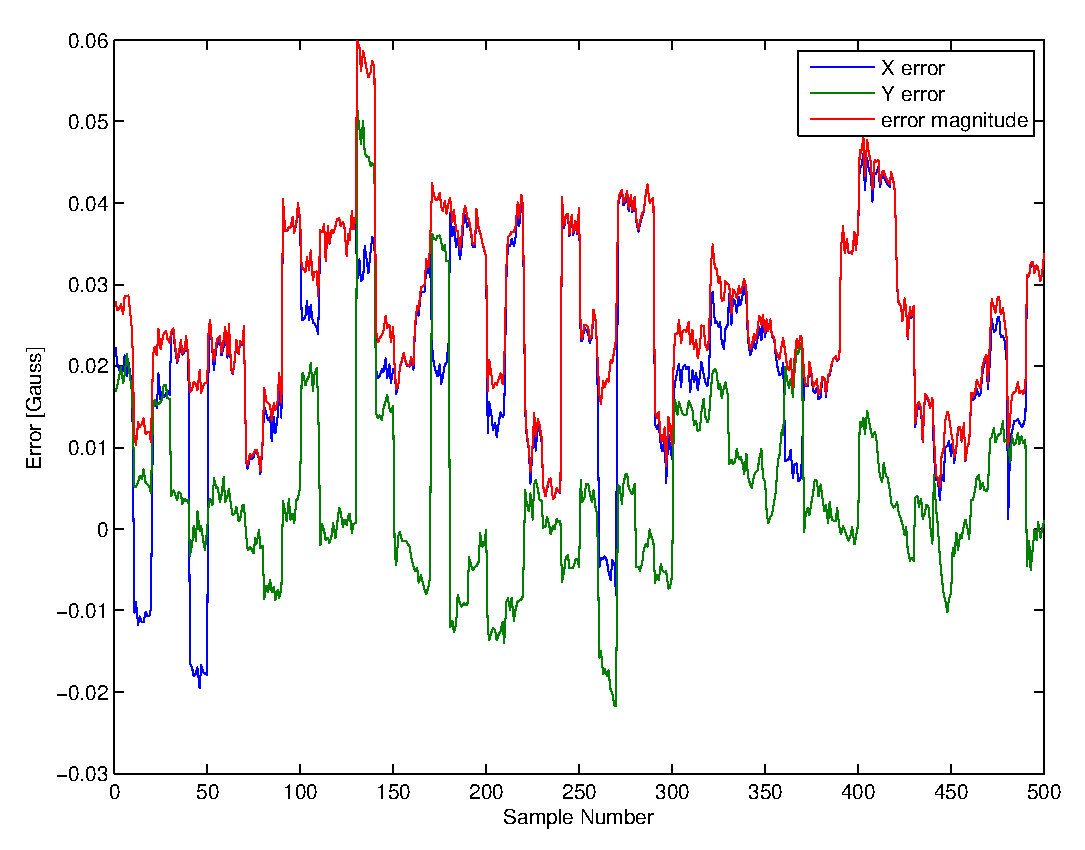
\includegraphics[width=0.8\linewidth]{torqueCalTst-err}
    \caption{Graph showing a torquer compensation error plot}
    \label{fig:tqerr}
\end{figure}

\subsection{Torquer Repeatability}

The torquer compensation method depends on the torquer offsets being repeatable. If the offsets are not very repeatable then the offsets will induce errors in the measured field. \Cref{fig:tqoff} shows a plot of the torquer offsets. The plot shows the offsets of the torquers when they are polarized in each direction. The offset for both of the magnetometer axes are shown. To create the plot each torquer was flipped 20 times in each direction. After each flip a magnetometer calibration was done to get the offset values. The offset values are normalized to show deviation from the median for better comparison. The maximum offset variation in \cref{fig:tqoff} is 20 mGauss.

The offset variations shown in \cref{fig:tqoff} are all less than the maximum error from \cref{fig:tqerr}. This is likely because the maximum offsets did not occur all at the same time.

\begin{figure}[!ht]
    \centering
    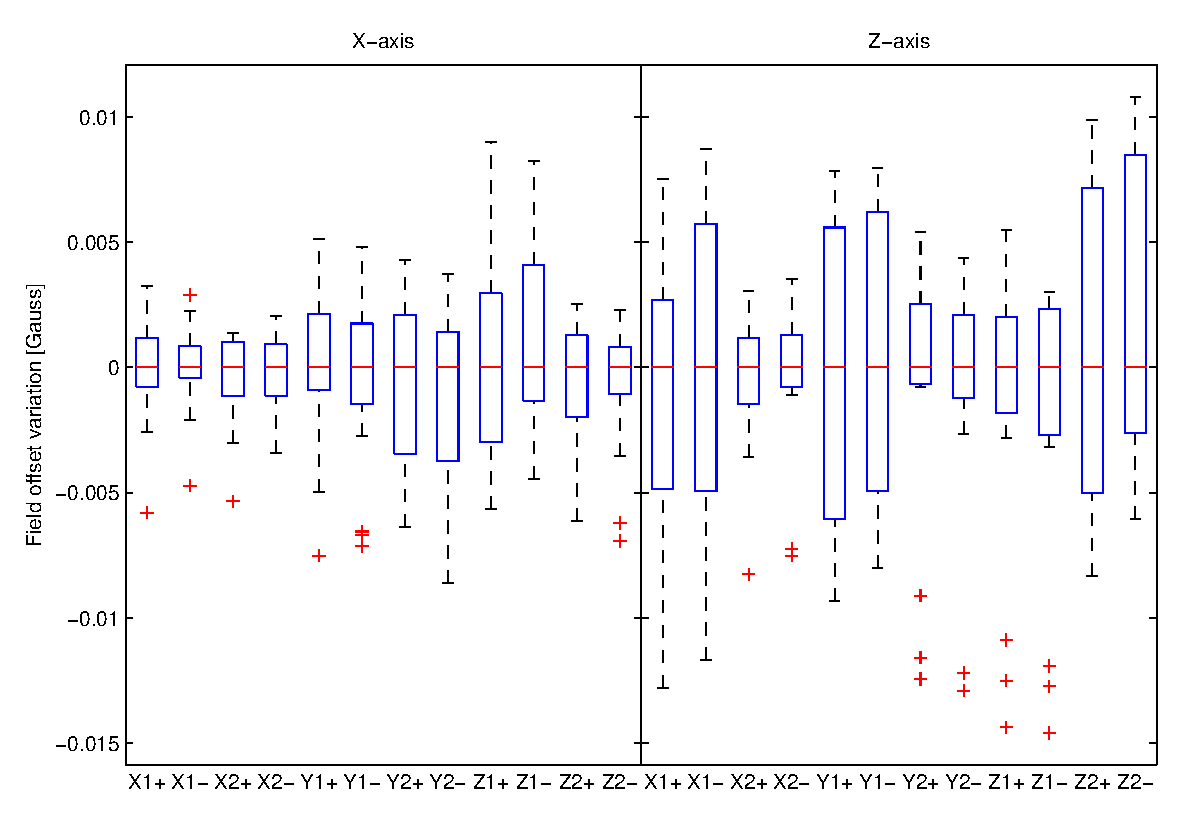
\includegraphics[width=0.9\linewidth]{torqueOffsets}
    \caption{Box Plot from torquer offset test}
    \label{fig:tqoff}
\end{figure}



\subsection{Gyro Verification}

\subsection{Feedback Verification}

To test the torquer feedback 

\section{\acl{ADS} Verification}

\section{Torquer Verification}

\subsection{Driver Verification}

To test the torquer drivers 


\section{Software Verification}

\section{System Verification}

Testing of torquer calibration

Magnetic interference from currents

